\chapter{Obsah odevzdaný na úložiště \textit{NextCloud}}
\label{chap:appendix-structure}
Tato kapitola znázorňuje strukturu odevzdaných souborů na úložišti \textit{NextCloud}.
\begin{verbatim}
.
|--- src
|   |---aggregate.py......(skript sloužící pro~agregaci dat z datových sad)
|   |--- config.py....................................(konfigurační soubor)
|   |--- data/...................................(složka s datovými sadami)
|   |   |--- gh-repos.md
|   |   |--- iscx.csv
|   |   |--- iscx-raw.csv
|   |   |-- mobile_desktop_apps_raw.csv
|   |--- identify/..............(složka s moduly pro identifikaci aplikací)
|   |   |--- command_line_parser.py..(zpracování parametrů příkazové řádky)
|   |   |--- database.py...(správa přístupu k datům a jejich strukturování)
|   |   |--- fingerprinting.py ........(identifikace spojení pomocí otisků)
|   |   |--- __init__.py
|   |   |--- ja_context.py.......................(kombinovaná identifikace)
|   |   |--- logger.py............................(logování chodu programu)
|   |   |-- pattern_matching.py...(implementace  PatternMatching a Apriori)
|   |--- main.py................................(hlavní spustitelný skript)
|   |--- Makefile............................(automatizace běžných příkazů)
|   |--- out/..............................(složka s výýsledky experiemntů)
|   |--- README.md...........................(popis a dokumentace projektu)
|   |-- requirements.txt.......................(seznam závislostí projektu)
|--- thesis-src/........................(zdrojové soubory technické zprávy)
|-- xpomsa00-BP.pdf......................................(technická zpráva)
\end{verbatim}

\chapter{Rozšířené seznámení s~datovými sadami a~strukturou}
\label{chp:appendix-ds}
V této části zprávy jsou uvedeny kompletní tabulky obsahující všechny atributy datových sad. Pro~úplnost a~transparentnost jsou všechny hodnoty, včetně jejich unikátních a~celkových počtů, uvedeny v~tabulkách bez~jakýchkoli úprav.

\section{Kompletní přehled hodnot v~datových sadách}
Tabulky jsou následující: Tabulka~\ref{tab:iscx-appendix} obsahuje přehled atributů v~datové sadě \texttt{iscx.csv}, tabulka~\ref{tab:iscx-raw-appendix} uvádí přehled atributů v~datové sadě \texttt{iscx-raw.csv} a~tabulka~\ref{tab:mobile-appendix} poskytuje přehled atributů v~datové sadě \texttt{mobile\_desktop\_apps\_raw.csv}.
\subsection{iscx.csv}
\begin{table}[H]
	\centering
	\begin{tabular}{lllll}
		\toprule
		\multicolumn{5}{c}{\texttt{iscx.csv}} \\
		\midrule
		\textbf{Atribut} & \textbf{Počet unikátních hodnot} & \textbf{( v~\%)} & \textbf{ Celkový počet} & \textbf{( v~\%)} \\
		\midrule
		SrcIP            & 17                                  & 0.70             & 2436                      & 100.00           \\
		DstIP            & 426                                 & 17.49            & 2436                      & 100.00           \\
		SrcPort          & 2297                                & 94.29            & 2436                      & 100.00           \\
		DstPort          & 159                                 & 6.53             & 2436                      & 100.00           \\
		SNI              & 207                                 & 8.50             & 2092                      & 85.88            \\
		OrgName          & 72                                  & 2.96             & 2300                      & 94.42            \\
		JA3hash          & 46                                  & 1.89             & 2436                      & 100.00           \\
		JA4hash          & 42                                  & 1.72             & 2436                      & 100.00           \\
		AppName          & 16                                  & 0.66             & 2436                      & 100.00           \\
		Type             & 2                                   & 0.08             & 2436                      & 100.00           \\
		JA3Shash         & 117                                 & 4.80             & 2399                      & 98.48            \\
		JA4Shash         & 127                                 & 5.21             & 2399                      & 98.48            \\
		Filename         & 109                                 & 4.47             & 2399                      & 98.48            \\
		Version          & 1                                   & 0.04             & 2399                      & 98.48            \\
		\bottomrule
	\end{tabular}
	\caption{Přehled všech atributů v~\texttt{iscx.csv}}
	\label{tab:iscx-appendix}
\end{table}
\newpage
\subsection{iscx-raw.csv}
\begin{table}[h!]
	\centering
	\begin{tabular}{lllll}
		\toprule
		\multicolumn{5}{c}{\texttt{iscx-raw.csv}} \\
		\midrule
		\textbf{Atribut}        & \textbf{Unikátní hodnoty} & \textbf{( v~\%)} & \textbf{Celkový počet} & \textbf{( v~\%)} \\
		\midrule
		SrcIP                   & 17                                  & 0.70             & 2436                     & 100.00           \\
		DstIP                   & 426                                 & 17.49            & 2436                     & 100.00           \\
		SrcPort                 & 2297                                & 94.29            & 2436                     & 100.00           \\
		DstPort                 & 159                                 & 6.53             & 2436                     & 100.00           \\
		Proto                   & 1                                   & 0.04             & 2436                     & 100.00           \\
		SNI                     & 207                                 & 8.50             & 2092                     & 85.88            \\
		OrgName                 & 72                                  & 2.96             & 2300                     & 94.42            \\
		TLSVersion              & 3                                   & 0.12             & 2436                     & 100.00           \\
		ClientCipherSuite       & 24                                  & 0.99             & 2436                     & 100.00           \\
		ClientExtensions        & 32                                  & 1.31             & 2436                     & 100.00           \\
		ClientSupportedGroups   & 5                                   & 0.21             & 2342                     & 96.14            \\
		EC\_fmt                 & 2                                   & 0.08             & 2342                     & 96.14            \\
		ALPN                    & 6                                   & 0.25             & 1310                     & 53.78            \\
		SignatureAlgorithms     & 8                                   & 0.33             & 2398                     & 98.44            \\
		ClientSupportedVersions & 0                                   & 0.00             & 0                        & 0.00             \\
		JA3hash                 & 46                                  & 1.89             & 2436                     & 100.00           \\
		JA4hash                 & 42                                  & 1.72             & 2436                     & 100.00           \\
		JA4\_raw                & 42                                  & 1.72             & 2436                     & 100.00           \\
		AppName                 & 16                                  & 0.66             & 2436                     & 100.00           \\
		Type                    & 2                                   & 0.08             & 2436                     & 100.00           \\
		ServerCipherSuite       & 22                                  & 0.90             & 2399                     & 98.48            \\
		ServerExtensions        & 45                                  & 1.85             & 2399                     & 98.48            \\
		ServerSupportedVersions & 0                                   & 0.00             & 0                        & 0.00             \\
		JA3Shash                & 117                                 & 4.80             & 2399                     & 98.48            \\
		JA4Shash                & 127                                 & 5.21             & 2399                     & 98.48            \\
		JA4S\_raw               & 127                                 & 5.21             & 2399                     & 98.48            \\
		Filename                & 109                                 & 4.47             & 2399                     & 98.48            \\
		Version                 & 1                                   & 0.04             & 2399                     & 98.48            \\
		\bottomrule
	\end{tabular}
	\caption{Přehled všech atributů v~\texttt{iscx-raw.csv}}
	\label{tab:iscx-raw-appendix}
\end{table}
\newpage


\subsection{mobile\_desktop\_apps\_raw.csv}
\begin{table}[h!]
	\centering
	\begin{tabular}{lllll}
		\toprule
		\multicolumn{5}{c}{\texttt{mobile\_desktop\_apps\_raw.csv}} \\
		\midrule
		\textbf{Atribut}        & \textbf{Unikátní hodnoty} & \textbf{( v~\%)} & \textbf{Celkový počet} & \textbf{( v~\%)} \\
		\midrule
		SrcIP                   & 1254                                & 5.89             & 21301                    & 100.00           \\
		DstIP                   & 1686                                & 7.92             & 21301                    & 100.00           \\
		SrcPort                 & 5823                                & 27.34            & 21301                    & 100.00           \\
		DstPort                 & 2                                   & 0.01             & 21301                    & 100.00           \\
		Proto                   & 2                                   & 0.01             & 21301                    & 100.00           \\
		SNI                     & 929                                 & 4.36             & 21259                    & 99.80            \\
		OrgName                 & 197                                 & 0.92             & 21273                    & 99.87            \\
		TLSVersion              & 1                                   & 0.00             & 21301                    & 100.00           \\
		ClientCipherSuite       & 36                                  & 0.17             & 21301                    & 100.00           \\
		ClientExtensions        & 10462                               & 49.12            & 21301                    & 100.00           \\
		ClientSupportedGroups   & 61                                  & 0.29             & 21301                    & 100.00           \\
		EC\_fmt                 & 2                                   & 0.01             & 20522                    & 96.34            \\
		ALPN                    & 9                                   & 0.04             & 19505                    & 91.57            \\
		SignatureAlgorithms     & 17                                  & 0.08             & 21301                    & 100.00           \\
		ClientSupportedVersions & 50                                  & 0.23             & 18938                    & 88.91            \\
		JA3hash                 & 10495                               & 49.27            & 21301                    & 100.00           \\
		JA4hash                 & 123                                 & 0.58             & 21301                    & 100.00           \\
		JA4\_raw                & 123                                 & 0.58             & 21301                    & 100.00           \\
		AppName                 & 78                                  & 0.37             & 21301                    & 100.00           \\
		Type                    & 2                                   & 0.01             & 21266                    & 99.84            \\
		ServerCipherSuite       & 11                                  & 0.05             & 21180                    & 99.43            \\
		ServerExtensions        & 56                                  & 0.26             & 21180                    & 99.43            \\
		ServerSupportedVersions & 2                                   & 0.01             & 15977                    & 75.01            \\
		JA3Shash                & 83                                  & 0.39             & 21180                    & 99.43            \\
		JA4Shash                & 103                                 & 0.48             & 21180                    & 99.43            \\
		JA4S\_raw               & 103                                 & 0.48             & 21180                    & 99.43            \\
		Filename                & 1746                                & 8.20             & 21180                    & 99.43            \\
		Version                 & 1                                   & 0.00             & 21180                    & 99.43            \\
		\bottomrule
	\end{tabular}
	\caption{Přehled všech atributů v~\texttt{mobile\_desktop\_apps\_raw.csv}}
	\label{tab:mobile-appendix}
\end{table}

\section{Kompletní přehled aplikací v~datových sadách}
Dále jsou uvedeny nezkrácené tabulky obsahující všechny aplikace v~daných datových sadách spolu s~jejich zastoupením.
Tabulky jsou následující:
\begin{itemize}
	\item~\ref{tab:mobile-apps-appendix} --  Přehled aplikací v~datové sadě \texttt{mobile\_desktop\_apps\_raw.csv}.
    
	\item~\ref{tab:iscx-apps-appendix} --  Přehled aplikací v~datové sadě \texttt{iscx.csv}.
\end{itemize}
\newpage
\subsection{Aplikace v~mobile\_desktop\_apps\_raw.csv}
\begin{table}[h!]
	\centering
	\begin{tabular}{llllll}
		\toprule
		\multicolumn{6}{c}{\texttt{mobile\_desktop\_apps\_raw.csv}} \\
		\midrule
		\textbf{App}   & \textbf{Počet} & \textbf{Podíl (\%)} & \textbf{App}       & \textbf{Počet} & \textbf{Podíl (\%)} \\
		\midrule
		AirDroidAirDroid    & 1774            & 8.33                 & google-play             & 135             & 0.63                 \\
		OerOer              & 1441            & 6.76                 & facebook                & 134             & 0.63                 \\
		BiduTerBox          & 1252            & 5.88                 & gmail                   & 130             & 0.61                 \\
		AdmntMessenger      & 1180            & 5.54                 & instagram               & 129             & 0.61                 \\
		accuweather         & 1052            & 4.94                 & mapy-cz                 & 108             & 0.51                 \\
		OenMedi4KStogrm     & 1020            & 4.79                 & viber                   & 100             & 0.47                 \\
		OenMedi4KTokkit     & 1012            & 4.75                 & LINELINE                & 95              & 0.45                 \\
		aliexpress          & 719             & 3.38                 & regiojet                & 94              & 0.44                 \\
		TemSonrrSonrr       & 717             & 3.37                 & snapchat                & 85              & 0.40                 \\
		MozillFirefox       & 637             & 2.99                 & signal                  & 83              & 0.39                 \\
		EstmobSendAnywhere  & 607             & 2.85                 & packeta                 & 82              & 0.38                 \\
		HedsetHedset        & 554             & 2.60                 & whatsapp                & 81              & 0.38                 \\
		EvernoteEvernote    & 469             & 2.20                 & TymnixEletorrent        & 79              & 0.37                 \\
		capcut              & 413             & 1.94                 & spotify                 & 78              & 0.37                 \\
		shein               & 368             & 1.73                 & CloudAGCloudDrive       & 78              & 0.37                 \\
		TIDALMusiASTIDAL    & 365             & 1.71                 & OenWhiserSystemsSignl   & 77              & 0.36                 \\
		BeeerBeeer          & 342             & 1.61                 & disney-plus             & 77              & 0.36                 \\
		RkutenViber         & 300             & 1.41                 & ZoomZoom                & 75              & 0.35                 \\
		temu                & 299             & 1.40                 & MirosoftEdge            & 75              & 0.35                 \\
		GoogleChrome        & 287             & 1.35                 & messenger               & 74              & 0.35                 \\
		waze                & 267             & 1.25                 & eMClienteMClient        & 72              & 0.34                 \\
		NotionNotion        & 263             & 1.23                 & TrillinTrillin          & 72              & 0.34                 \\
		DeezerDeezer        & 262             & 1.23                 & YndexMessenger          & 72              & 0.34                 \\
		MozillThunderbird   & 253             & 1.19                 & ProtonProtonDrive       & 72              & 0.34                 \\
		AsnAsn              & 248             & 1.16                 & CozyCloudCozyDrive      & 72              & 0.34                 \\
		CrineCrine          & 232             & 1.09                 & netflix                 & 71              & 0.33                 \\
		tiktok              & 217             & 1.02                 & twitter                 & 64              & 0.30                 \\
		SlkTehnologiesSlk   & 214             & 1.00                 & reddit                  & 54              & 0.25                 \\
		trello              & 205             & 0.96                 & wechat                  & 54              & 0.25                 \\
		SotifySotify        & 199             & 0.93                 & discord                 & 50              & 0.23                 \\
		wolt                & 179             & 0.84                 & muj-vlak                & 46              & 0.22                 \\
		alipay              & 177             & 0.83                 & NextloudNextloudDeskto  & 36              & 0.17                 \\
		alza                & 167             & 0.78                 & MehediHssnTweeten       & 36              & 0.17                 \\
		BrveBrve            & 150             & 0.70                 & MegMEGASyn              & 35              & 0.16                 \\
		NotionNotionClendr  & 145             & 0.68                 & SlshedIoInssist         & 27              & 0.13                 \\
		chatgpt             & 144             & 0.68                 & TemDriveSystemsTemDrive & 21              & 0.10                 \\
		foodora             & 142             & 0.67                 & MilbirdMilbird          & 15              & 0.07                 \\
		BiglySoftwreBiglyBT & 141             & 0.66                 & telegram                & 12              & 0.06                 \\
		youtube             & 137             & 0.64                 & TelegrmTelegrmDeskto    & 1               & 0.00                 \\
		\bottomrule
	\end{tabular}
	\caption{Přehled všech aplikací v~\texttt{mobile\_desktop\_apps\_raw.csv}}
	\label{tab:mobile-apps-appendix}
\end{table}
\newpage
\subsection{Aplikace v~iscx.csv}
\begin{table}[h!]
	\centering
	\begin{tabular}{lll}
		\toprule
		\multicolumn{3}{c}{\texttt{iscx.csv}} \\
		\midrule
		\textbf{Aplikace} & \textbf{Počet} & \textbf{Podíl (\%)} \\
		\midrule
		hangout           & 553             & 22.70                \\
		skype             & 436             & 17.90                \\
		email             & 315             & 12.93                \\
		facebook          & 229             & 9.40                 \\
		ftps              & 229             & 9.40                 \\
		vimeo             & 211             & 8.66                 \\
		youtube           & 209             & 8.58                 \\
		voipbuster        & 64              & 2.63                 \\
		spotify           & 60              & 2.46                 \\
		netflix           & 39              & 1.60                 \\
		gmail             & 35              & 1.44                 \\
		sftp              & 21              & 0.86                 \\
		aim               & 11              & 0.45                 \\
		scp               & 9               & 0.37                 \\
		bittorrent        & 8               & 0.33                 \\
		icq               & 7               & 0.29                 \\
		\bottomrule
	\end{tabular}
	\caption{Přehled všech aplikací v~\texttt{iscx.csv}}
	\label{tab:iscx-apps-appendix}
\end{table}

\chapter{Rozšířený diagram tříd} 
\label{chp:appendix-class-diagram}

Tento diagram~\ref{fig:appendix-class} tříd byl automaticky vygenerován pomocí nástroje \texttt{pyreverse}, který je součástí balíku \texttt{pylint}. Diagram vizuálně zachycuje strukturu systému, hierarchii tříd a~jejich vzájemné vztahy, včetně dědičnosti a~závislostí.

\begin{figure}[H]
    \centering
    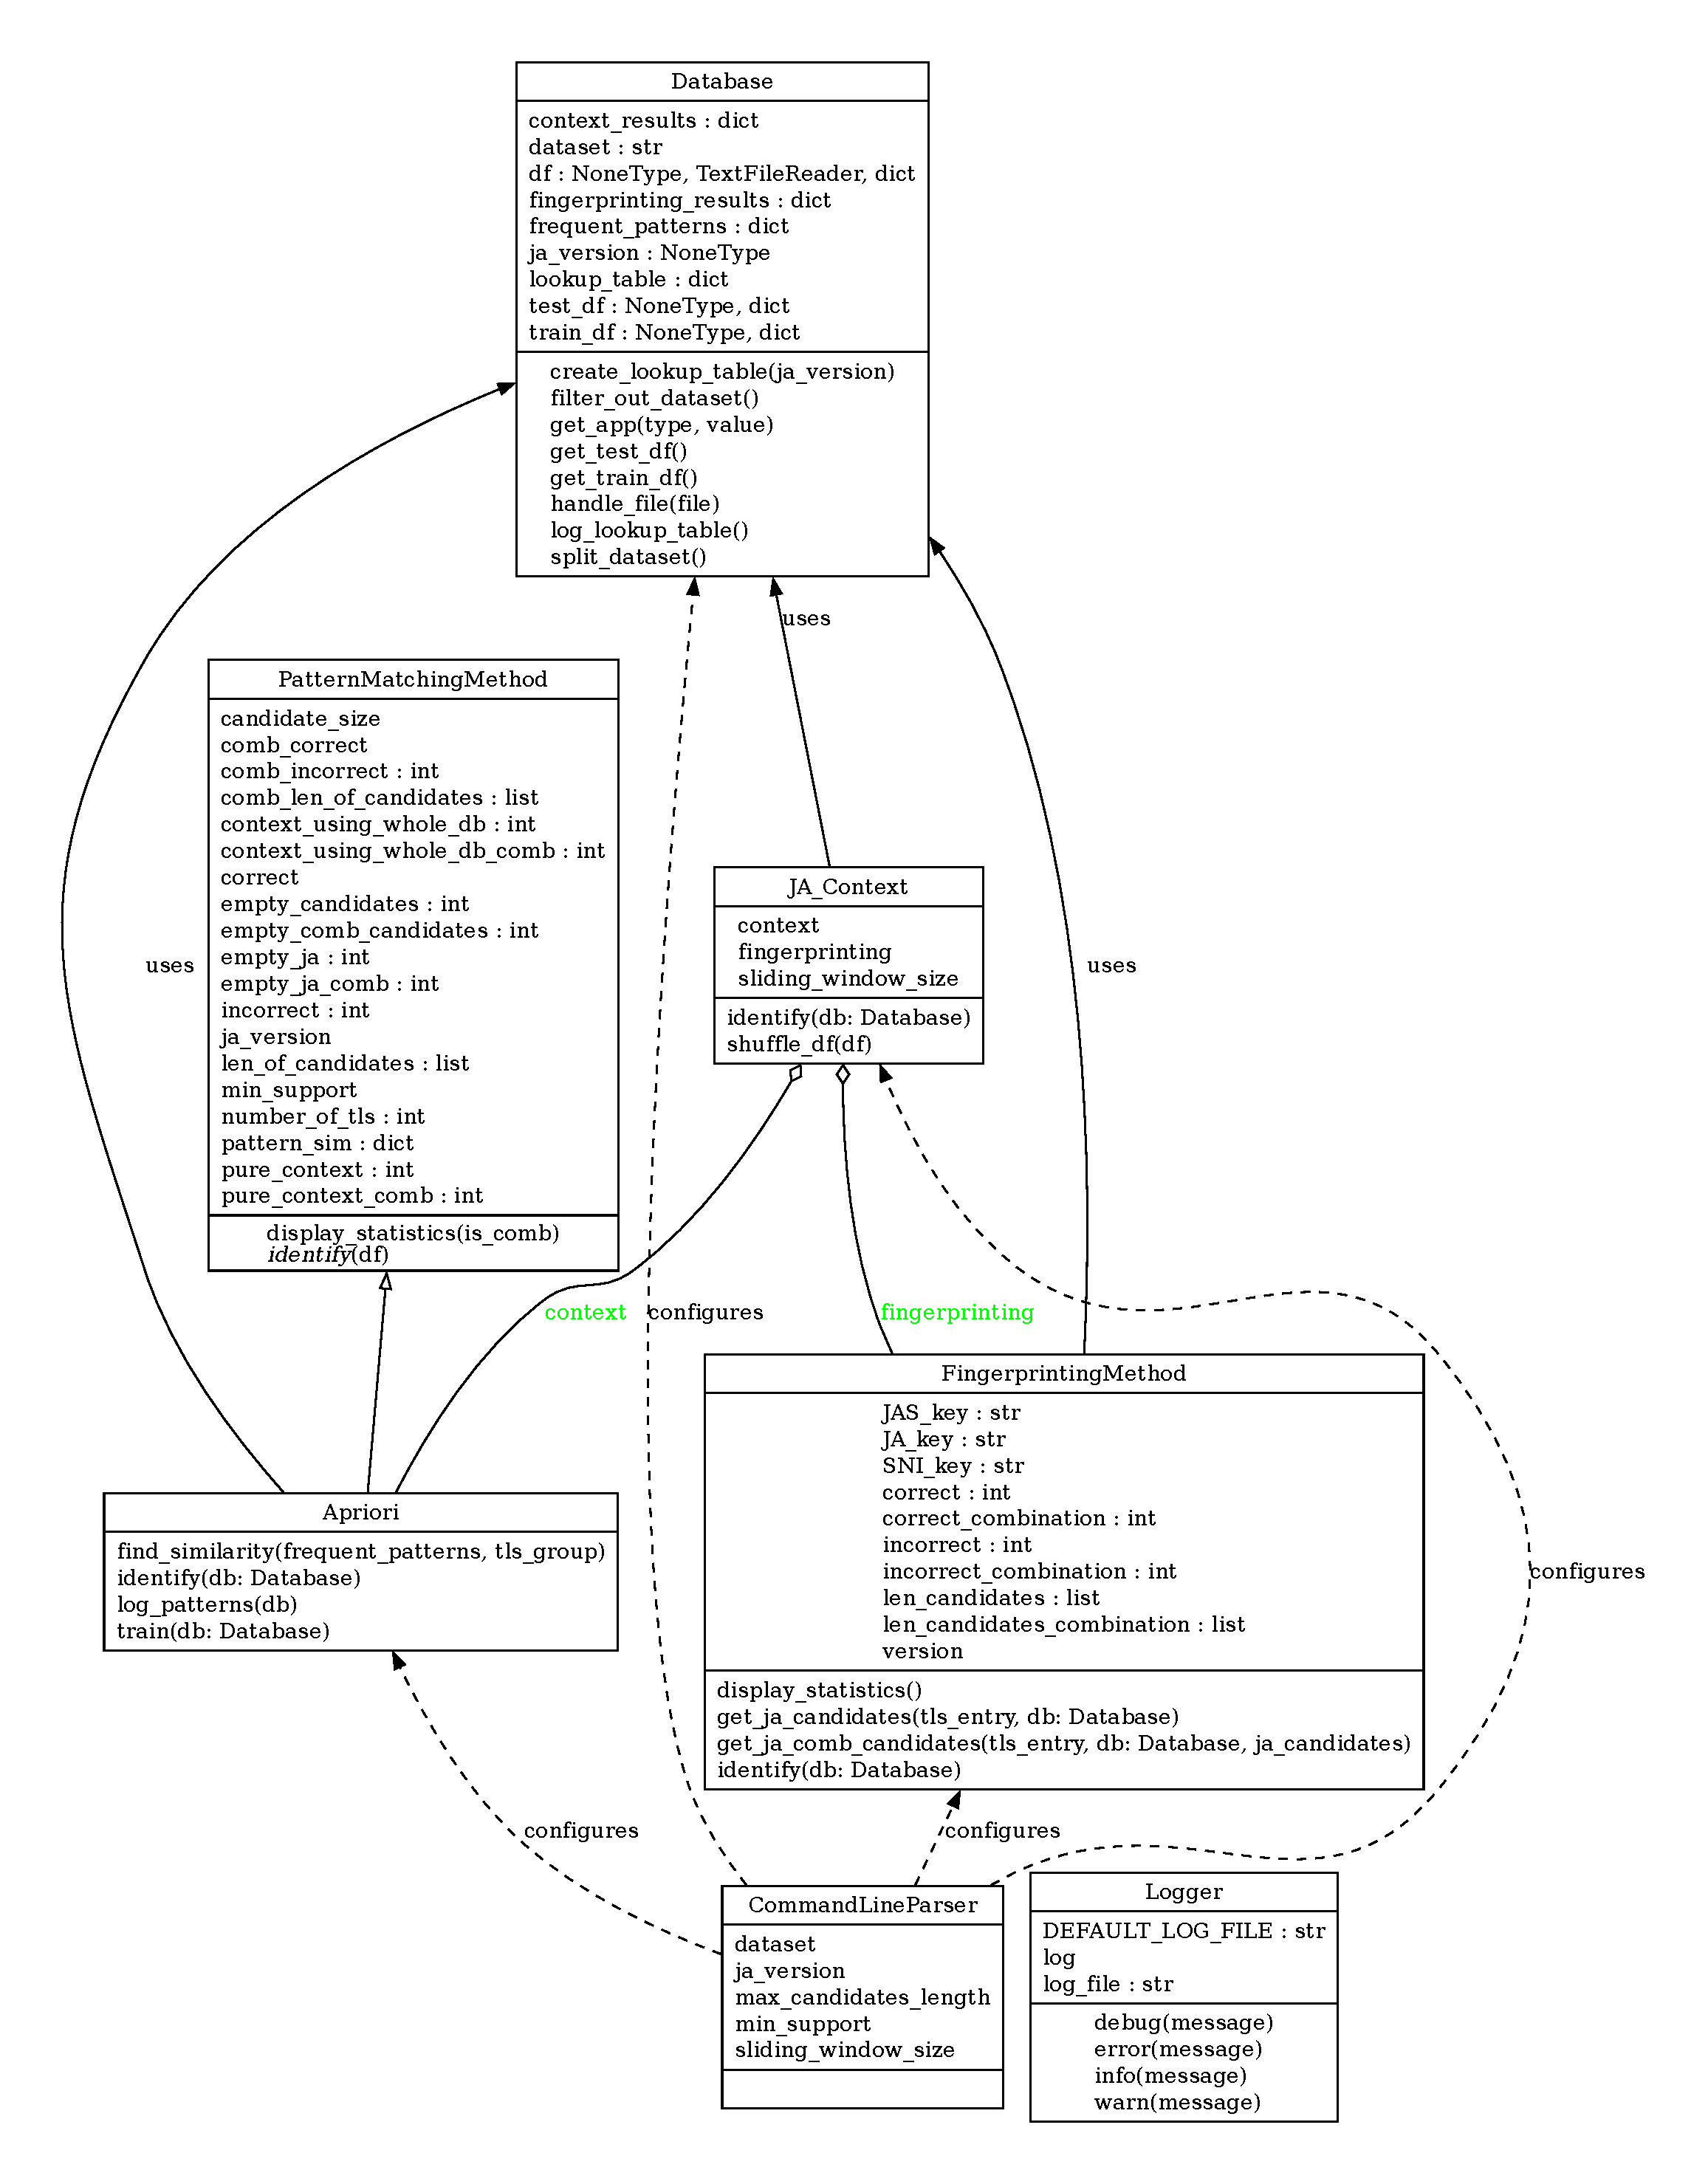
\includegraphics[width=0.7\textwidth]{obrazky-figures/class-dia-generated.pdf}
    \caption{Rozšířený diagram tříd}
    \label{fig:appendix-class}
\end{figure}

\chapter{Rozšířené výsledky experimentů}
\label{chp:appendix-experiments}
Tato kapitola obsahuje podrobné výstupy z~provedených experimentů. Jsou zde uvedeny grafy, tabulky a~další doplňující materiály, sloužící k~hlubší analýze a~interpretaci dosažených výsledků.

\section{Experiment 1}
\label{sec:appendix:ex1}

Následují neupravené a~nezkrácené tabulky uvádějící přesnost, průměrnou délku a~čas potřebný k~identifikaci pro~všechny testované kombinace.

\begin{table}[H]
    \centering
	\begin{tabular}{lrrrrr}
		\toprule
        \multicolumn{6}{c}{\textbf{Zúžení databáze kandidátů pomocí JA3}} \\
        \midrule
		\multirow{2}*{\textbf{Kombinace položek}}&\multicolumn{2}{c}{\texttt{iscx.csv}} & \multicolumn{3}{c}{\texttt{mobile\_desktop\_apps\_raw.csv}} \\
		                  & \textbf{Přesnost} & \textbf{Délka} & \textbf{Přesnost} & \textbf{Délka} & \textbf{Čas[s]} \\
		\midrule
		JA3               & 0.837              & 2.128           & 0.279              & 2.778           & 74.470        \\
		JA4               & 0.837              & 2.128           & 0.390              & 2.792           & 60.340        \\
		JA3+JA4           & 0.837              & 2.128           & 0.298              & 2.796           & 98.680        \\
		JA3+JA3S          & 0.847              & 2.128           & 0.365              & 2.796           & 101.050       \\
		JA4+JA4S          & 0.842              & 2.128           & 0.487              & 2.796           & 112.910       \\
		JA3+JA3S+SNI      & 0.852              & 2.128           & 0.371              & 2.796           & 163.680       \\
		JA4+JA4S+SNI      & 0.847              & 2.128           & 0.490              & 2.796           & 185.050       \\
		JA34S*            & 0.842              & 2.128           & 0.444              & 2.796           & 363.750       \\
		JA34S*+SNI        & 0.842              & 2.128           & 0.441              & 2.796           & 575.500       \\
		JA34S*+SNI+ORG    & 0.849              & 2.128           & 0.423              & 2.796           & 1123.730      \\
		JA34S*+SNI+ORG+CE & 0.849              & 2.128           & 0.379              & 2.796           & 2157.100      \\
		
		\bottomrule
	\end{tabular}
	\caption{Výsledky experimentu s~kombinacemi položek při~zúžení databáze kandidátů pomocí otisku \textit{JA3}}
	\label{tab:appendix-merged-not_comb-accuracy-ja3}
\end{table}

\begin{table}[H]
    \centering
	\begin{tabular}{lrrrrr}
		\toprule
        \multicolumn{6}{c}{\textbf{Zúžení databáze kandidátů pomocí JA4}} \\
        \midrule
		\multirow{2}*{\textbf{Kombinace položek}}&\multicolumn{2}{c}{\texttt{iscx.csv}} & \multicolumn{3}{c}{\texttt{mobile\_desktop\_apps\_raw.csv}} \\
		                  & \textbf{Přesnost} & \textbf{Délka} & \textbf{Přesnost} & \textbf{Délka} & \textbf{Čas[s]} \\
		\midrule
		JA3               & 0.837              & 2.128           & 0.304              & 2.781           & 53.660        \\
		JA4               & 0.837              & 2.128           & 0.387              & 2.785           & 32.340        \\
		JA3+JA4           & 0.837              & 2.128           & 0.361              & 2.789           & 48.100        \\
		JA3+JA3S          & 0.847              & 2.128           & 0.507              & 2.791           & 46.220        \\
		JA4+JA4S          & 0.842              & 2.128           & 0.558              & 2.791           & 58.500        \\
		JA3+JA3S+SNI      & 0.852              & 2.128           & 0.489              & 2.791           & 66.340        \\
		JA4+JA4S+SNI      & 0.847              & 2.128           & 0.548              & 2.791           & 84.030        \\
		JA34S*            & 0.842              & 2.128           & 0.577              & 2.791           & 150.820       \\
		JA34S*+SNI        & 0.842              & 2.128           & 0.549              & 2.791           & 225.220       \\
		JA34S*+SNI+ORG    & 0.849              & 2.128           & 0.533              & 2.791           & 400.770       \\
		JA34S*+SNI+ORG+CE & 0.849              & 2.128           & 0.507              & 2.791           & 840.660       \\
		
		\bottomrule
	\end{tabular}
	\caption{Výsledky experimentu s~kombinacemi položek při~zúžení databáze kandidátů pomocí otisku \textit{JA4}}
	\label{tab:appendix-merged-not_comb-accuracy-ja4}
\end{table}

\begin{table}[H]
    \centering
	\begin{tabular}{lrrrrr}
		\toprule
        \multicolumn{6}{c}{\textbf{Zúžení databáze kandidátů pomocí JA3+JA3S+SNI}} \\
        \midrule
		\multirow{2}*{\textbf{Kombinace položek}}&\multicolumn{2}{c}{\texttt{iscx.csv}} & \multicolumn{3}{c}{\texttt{mobile\_desktop\_apps\_raw.csv}} \\
		                  & \textbf{Přesnost} & \textbf{Délka} & \textbf{Přesnost} & \textbf{Délka} & \textbf{Čas[s]} \\
		\midrule
		JA3               & 0.867              & 1.583           & 0.385              & 2.287           & 74.470        \\
		JA4               & 0.867              & 1.583           & 0.771              & 1.747           & 60.340        \\
		JA3+JA4           & 0.872              & 1.583           & 0.764              & 1.745           & 98.680        \\
		JA3+JA3S          & 0.872              & 1.583           & 0.793              & 1.734           & 101.050       \\
		JA4+JA4S          & 0.869              & 1.583           & 0.800              & 1.734           & 112.910       \\
		JA3+JA3S+SNI      & 0.872              & 1.583           & 0.790              & 1.734           & 163.680       \\
		JA4+JA4S+SNI      & 0.867              & 1.583           & 0.798              & 1.734           & 185.050       \\
		JA34S*            & 0.867              & 1.583           & 0.793              & 1.734           & 363.750       \\
		JA34S*+SNI        & 0.867              & 1.583           & 0.792              & 1.734           & 575.500       \\
		JA34S*+SNI+ORG    & 0.869              & 1.583           & 0.774              & 1.734           & 1123.730      \\
		JA34S*+SNI+ORG+CE & 0.869              & 1.583           & 0.761              & 1.734           & 2157.100      \\
		
		\bottomrule
	\end{tabular}
	\caption{Výsledky experimentu s~kombinacemi položek při~zúžení databáze kandidátů pomocí kombinace  \textit{JA3+JA3S+SNI}}
	\label{tab:appendix-merged-comb-accuracy-ja3}
\end{table}


\begin{table}[H]
    \centering
	\begin{tabular}{lrrrrr}
		\toprule
        \multicolumn{6}{c}{\textbf{Zúžení databáze kandidátů pomocí JA4+JA4S+SNI}} \\
        \midrule
		\multirow{2}*{\textbf{Kombinace položek}}&\multicolumn{2}{c}{\texttt{iscx.csv}} & \multicolumn{3}{c}{\texttt{mobile\_desktop\_apps\_raw.csv}} \\
		                  & \textbf{Přesnost} & \textbf{Délka} & \textbf{Přesnost} & \textbf{Délka} & \textbf{Čas[s]} \\
		\midrule
		JA3               & 0.869              & 1.585           & 0.385              & 2.277           & 53.660        \\
		JA4               & 0.869              & 1.585           & 0.770              & 1.727           & 32.340        \\
		JA3+JA4           & 0.869              & 1.585           & 0.768              & 1.726           & 48.100        \\
		JA3+JA3S          & 0.874              & 1.585           & 0.793              & 1.714           & 46.220        \\
		JA4+JA4S          & 0.869              & 1.585           & 0.798              & 1.714           & 58.500        \\
		JA3+JA3S+SNI      & 0.874              & 1.585           & 0.795              & 1.714           & 66.340        \\
		JA4+JA4S+SNI      & 0.869              & 1.585           & 0.804              & 1.714           & 84.030        \\
		JA34S*            & 0.869              & 1.585           & 0.795              & 1.714           & 150.820       \\
		JA34S*+SNI        & 0.869              & 1.585           & 0.797              & 1.714           & 225.220       \\
		JA34S*+SNI+ORG    & 0.872              & 1.585           & 0.782              & 1.714           & 400.770       \\
		JA34S*+SNI+ORG+CE & 0.872              & 1.585           & 0.774              & 1.714           & 840.660       \\
		
		\bottomrule
	\end{tabular}
	\caption{Výsledky experimentu s~kombinacemi položek při~zúžení databáze kandidátů pomocí kombinace  \textit{JA4+JA4S+SNI}}
	\label{tab:appendix-merged-comb-accuracy-ja4}
\end{table}

\section{Experiment 2}
\label{sec:appendix:ex2}

Zde jsou uvedeny heatmapy znázorňující výsledky při~použití otisků \texttt{JA4} jako základní metody pro~generování počáteční kandidátní množiny.

\begin{figure}[H]
    \centering
    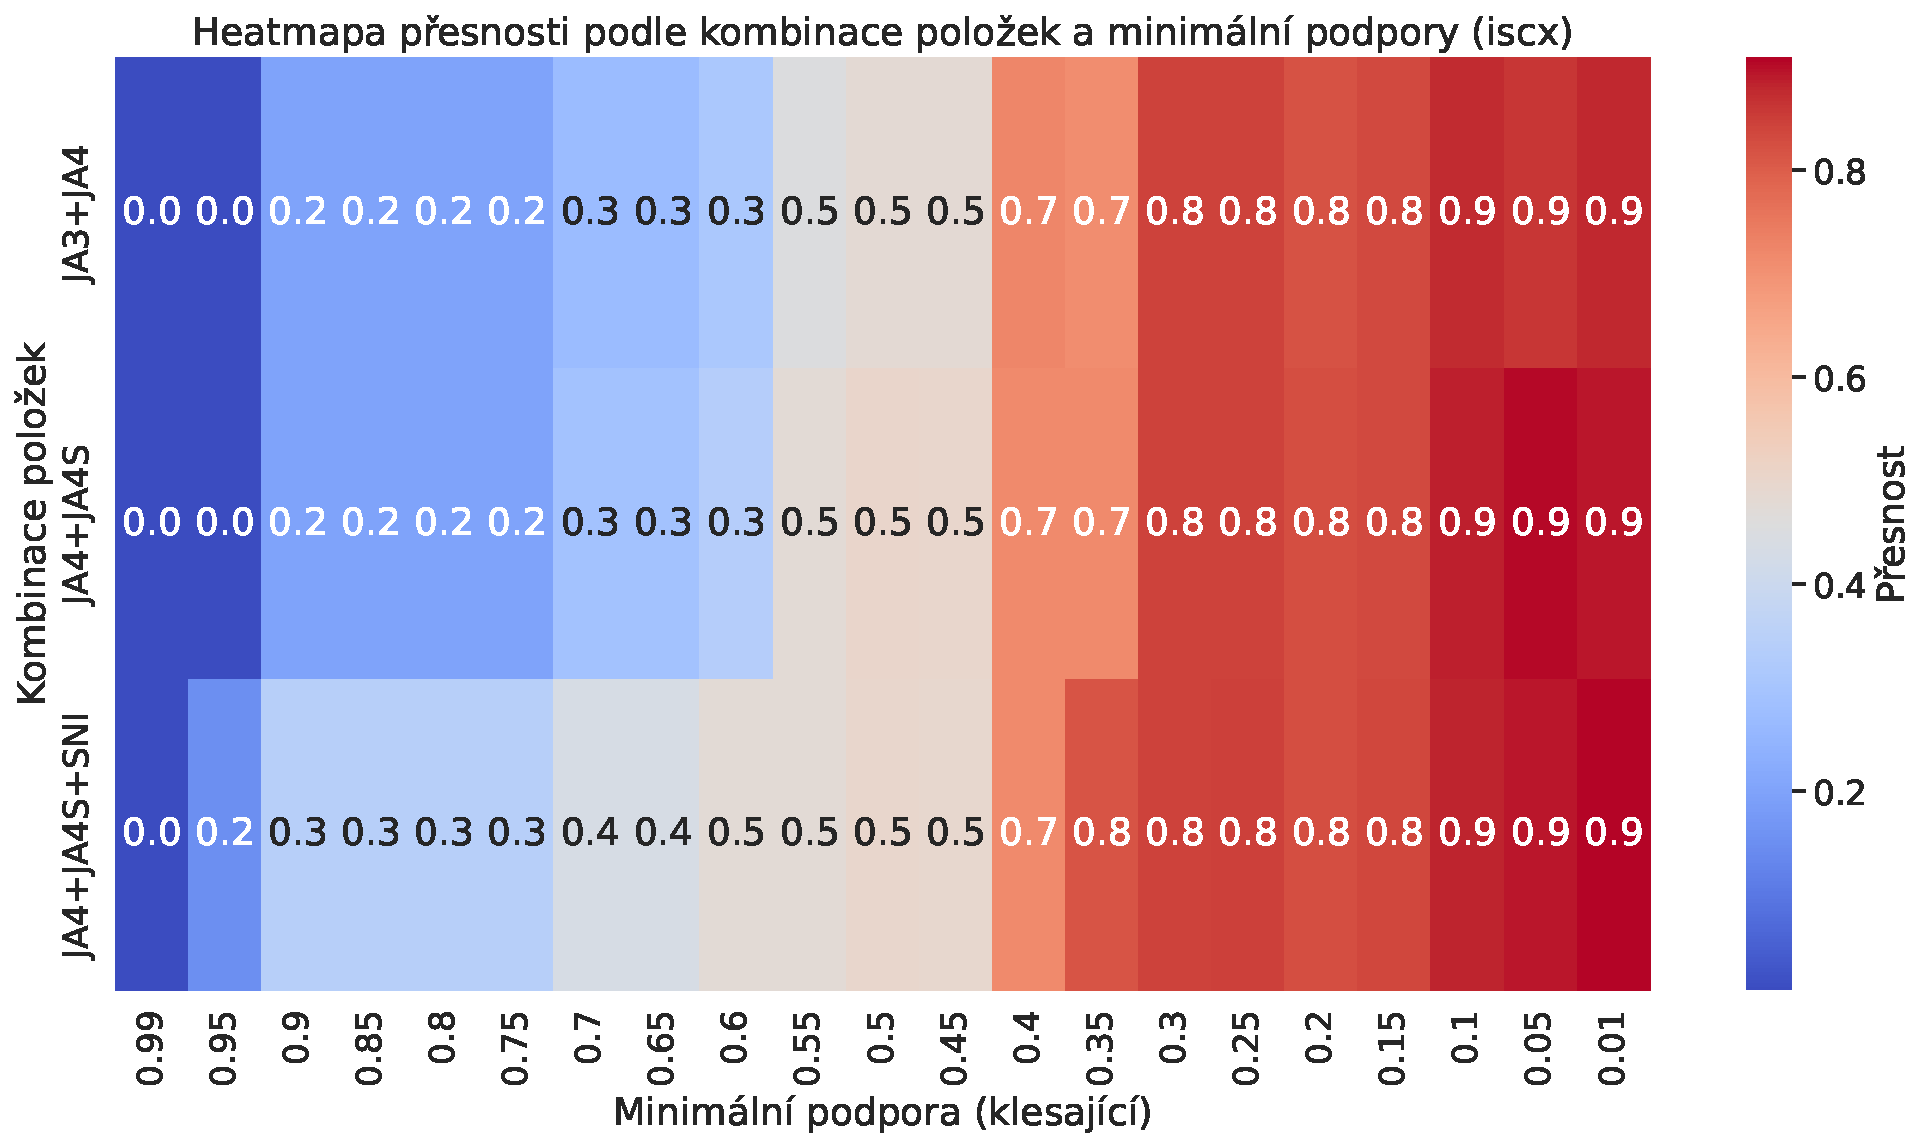
\includegraphics[width=\linewidth]{obrazky-figures/exps/ex2-iscx-heatmap_not_comb.pdf}
    \caption{Heatmapa zobrazující testované kombinace položek v~závislosti na~volbě minimální podpory a~dosažené přesnosti pro~datovou sadu \texttt{iscx.csv} při~použití otisků \textit{JA4}. }
    \label{fig:appendix-heatmap-iscx}
\end{figure}

\begin{figure}[H]
    \centering
    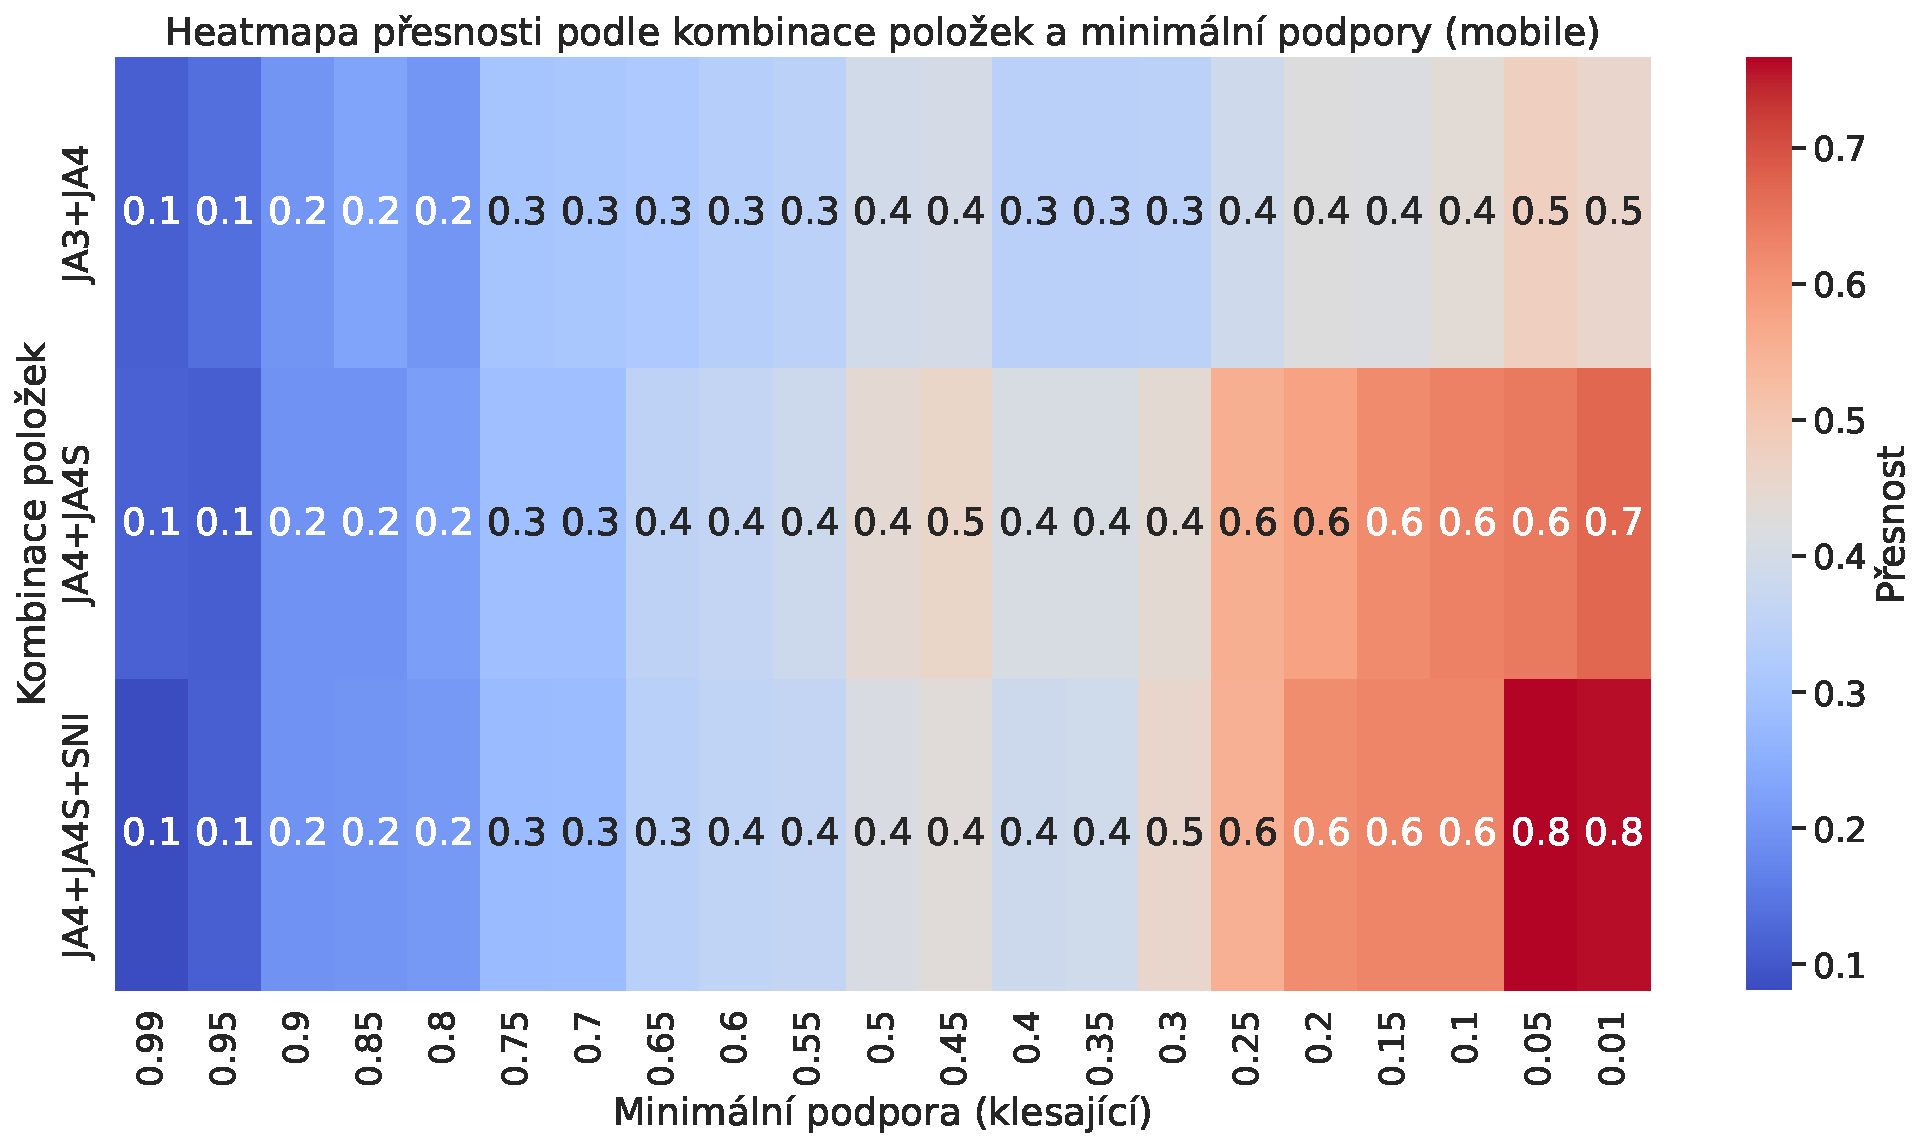
\includegraphics[width=\linewidth]{obrazky-figures/exps/ex2-mobile-heatmap_not_comb.pdf}
    \caption{Heatmapa zobrazující testované kombinace položek v~závislosti na~volbě minimální podpory a~dosažené přesnosti pro~datovou sadu \texttt{mobile desktop apps raw.csv} při~použití otisků \textit{JA4}. }
    \label{fig:appendix-heatmap-mobile}
\end{figure}

\begin{figure}[H]
    \centering
    \begin{minipage}[t]{0.49\textwidth}
        \centering
    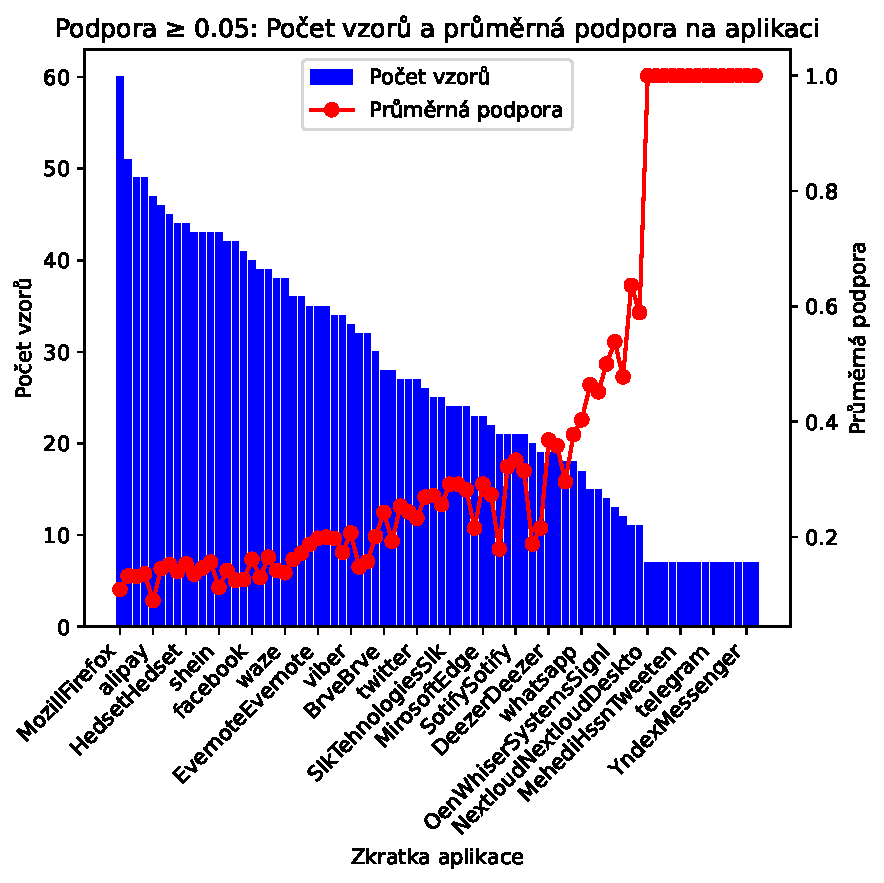
\includegraphics[width=\linewidth]{obrazky-figures/exps/patterns_support_0.05_mobile.pdf}
    \caption{Počet vzorů a~průměrná podpora na~aplikaci pro~\texttt{mobile desktop apps raw.csv} při~minimální podpoře 0.05.}
    \label{fig:appendix-}
    \end{minipage}%
    \hfill
    \begin{minipage}[t]{0.49\textwidth}
       \centering
        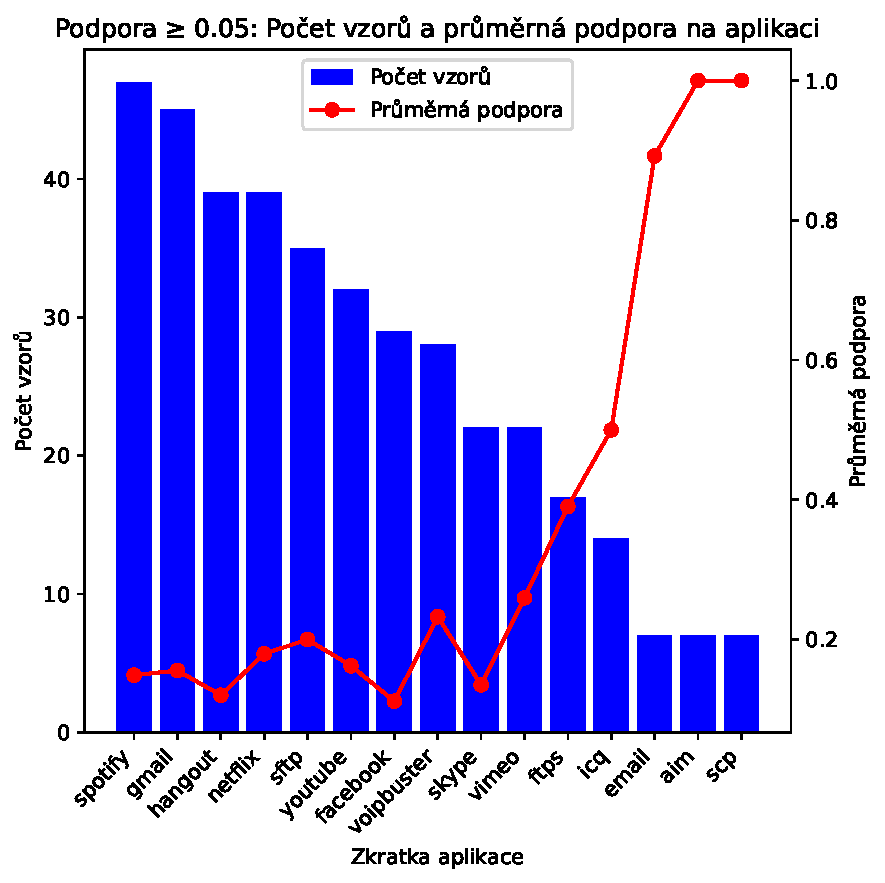
\includegraphics[width=\linewidth]{obrazky-figures/exps/patterns_support_0.05_iscx.pdf}
        \caption{Počet vzorů a~průměrná podpora na~aplikaci pro~\texttt{iscx.csv} při~minimální podpoře 0.05.}
        \label{fig:appendix-}
    \end{minipage}
\end{figure}

\begin{figure}[H]
    \centering
    \begin{minipage}[t]{0.49\textwidth}
        \centering
    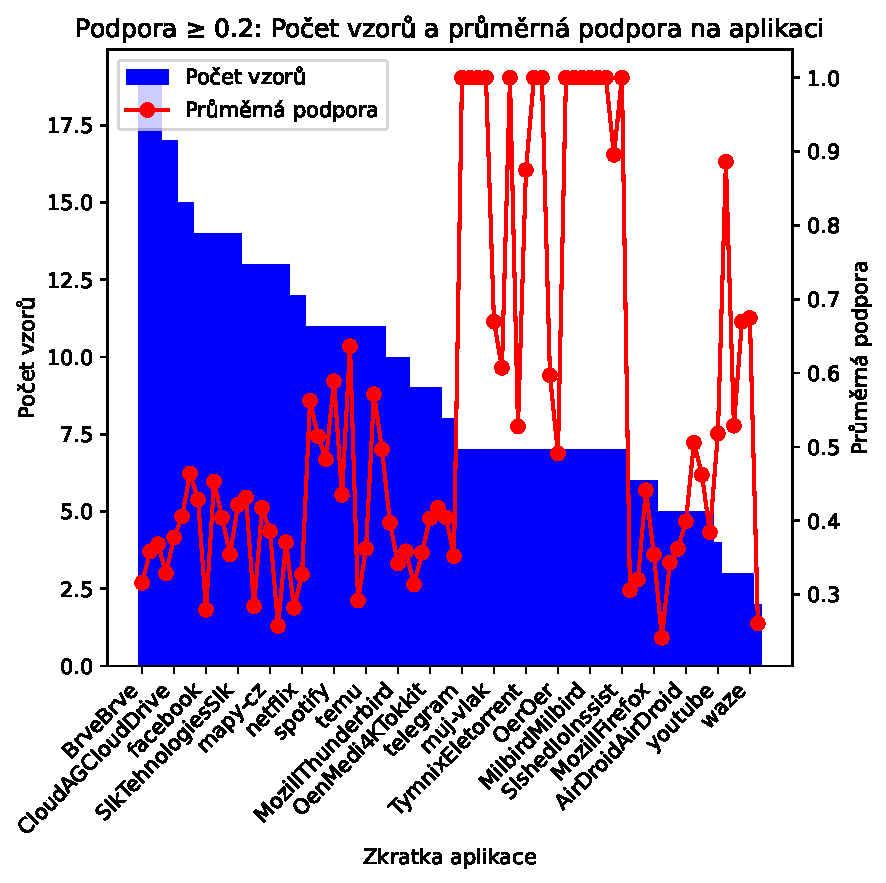
\includegraphics[width=\linewidth]{obrazky-figures/exps/patterns_support_0.2_mobile.pdf}
    \caption{Počet vzorů a~průměrná podpora na~aplikaci pro~\texttt{mobile desktop apps raw.csv} při~minimální podpoře 0.2.}
    \label{fig:appendix-}
    \end{minipage}%
    \hfill
    \begin{minipage}[t]{0.49\textwidth}
       \centering
        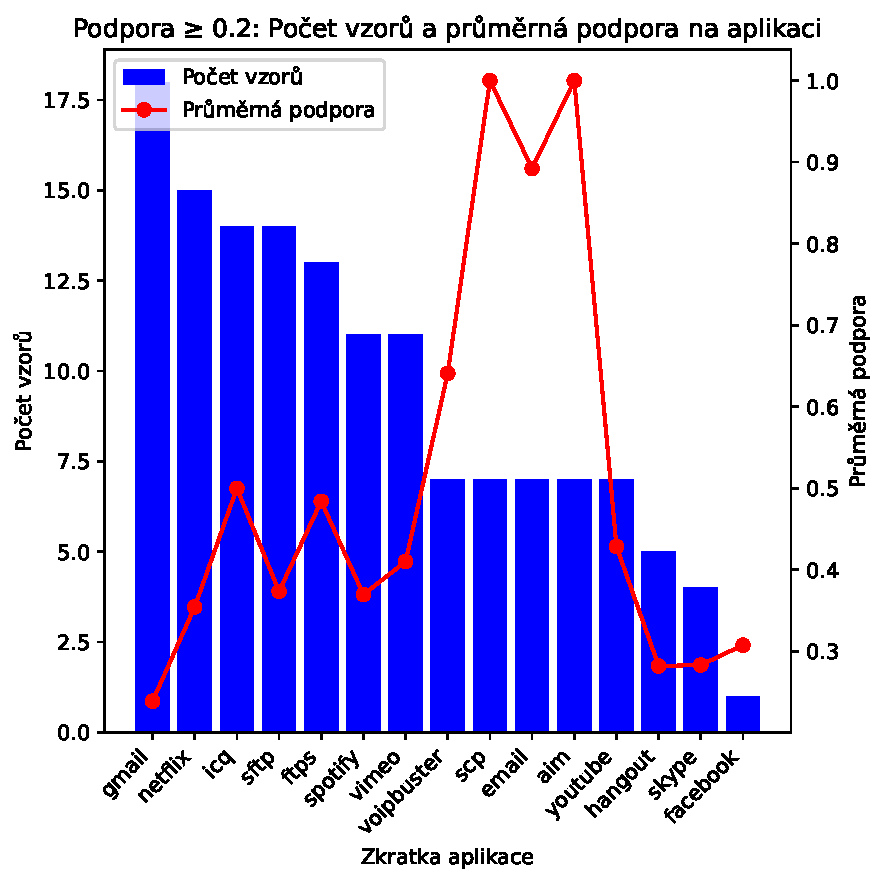
\includegraphics[width=\linewidth]{obrazky-figures/exps/patterns_support_0.2_iscx.pdf}
        \caption{Počet vzorů a~průměrná podpora na~aplikaci pro~\texttt{iscx.csv} při~minimální podpoře 0.2.}
        \label{fig:appendix-}
    \end{minipage}
\end{figure}

\begin{figure}[H]
    \centering
    \begin{minipage}[t]{0.49\textwidth}
        \centering
    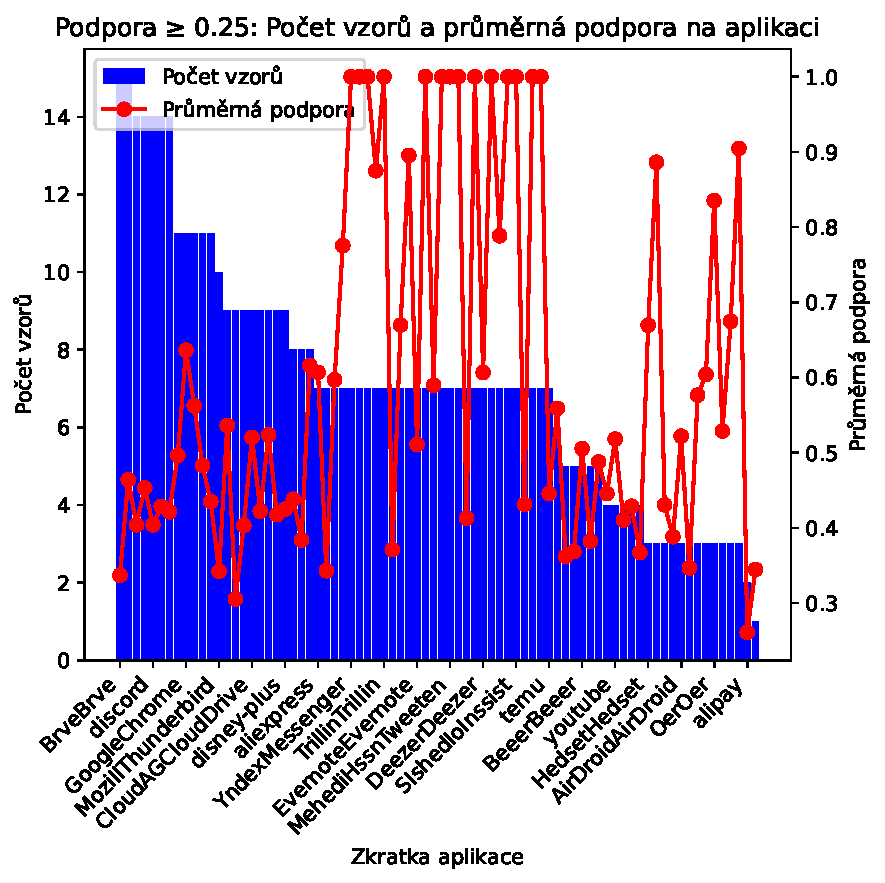
\includegraphics[width=\linewidth]{obrazky-figures/exps/patterns_support_0.25_mobile.pdf}
    \caption{Počet vzorů a~průměrná podpora na~aplikaci pro~\texttt{mobile desktop apps raw.csv} při~minimální podpoře 0.25.}
    \label{fig:appendix-}
    \end{minipage}%
    \hfill
    \begin{minipage}[t]{0.49\textwidth}
       \centering
        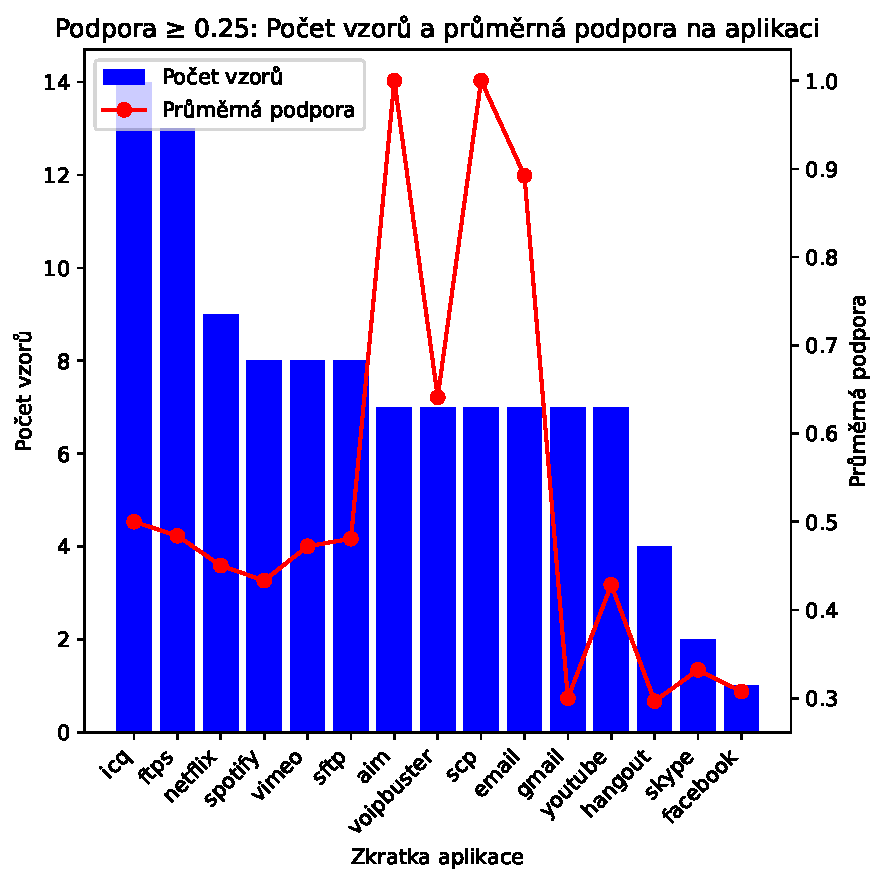
\includegraphics[width=\linewidth]{obrazky-figures/exps/patterns_support_0.25_iscx.pdf}
        \caption{Počet vzorů a~průměrná podpora na~aplikaci pro~\texttt{iscx.csv} při~minimální podpoře 0.25.}
        \label{fig:appendix-}
    \end{minipage}
\end{figure}

\begin{figure}[H]
    \centering
    \begin{minipage}[t]{0.49\textwidth}
        \centering
    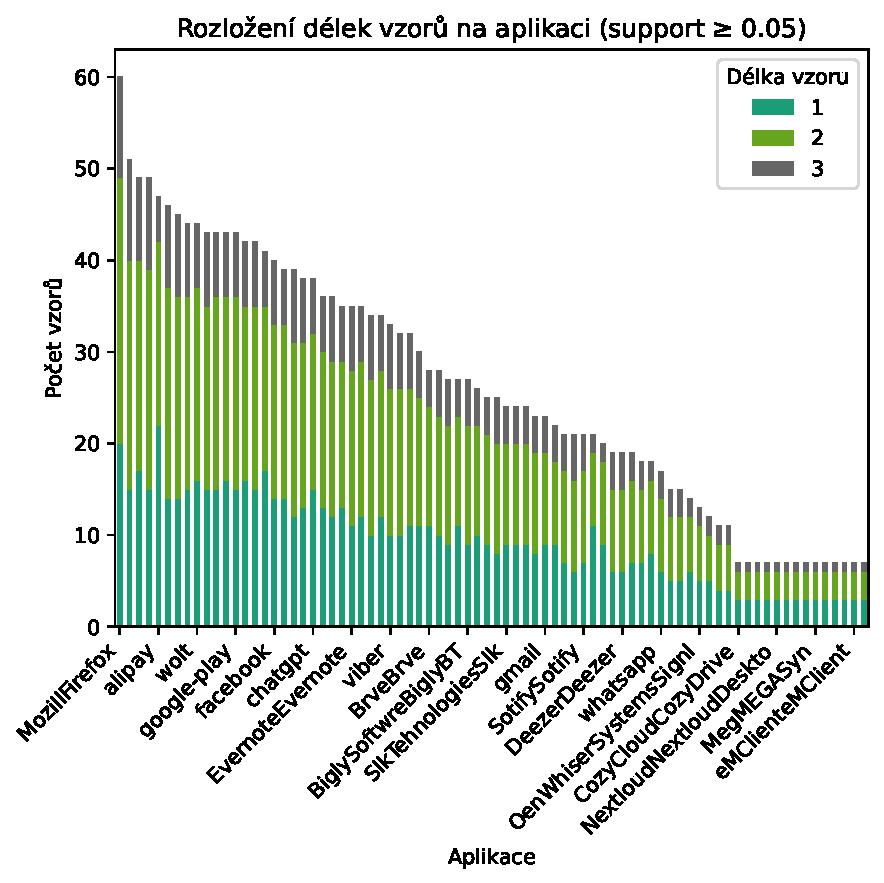
\includegraphics[width=\linewidth]{obrazky-figures/exps/pattern_lengths_0.05_mobile.pdf}
        \caption{Počet vzorů a~rozložení délek vzoru na~aplikaci pro~\texttt{mobile desktop apps raw.csv} při~minimální podpoře 0.05.}
    \label{fig:appendix-}
    \end{minipage}%
    \hfill
    \begin{minipage}[t]{0.49\textwidth}
       \centering
        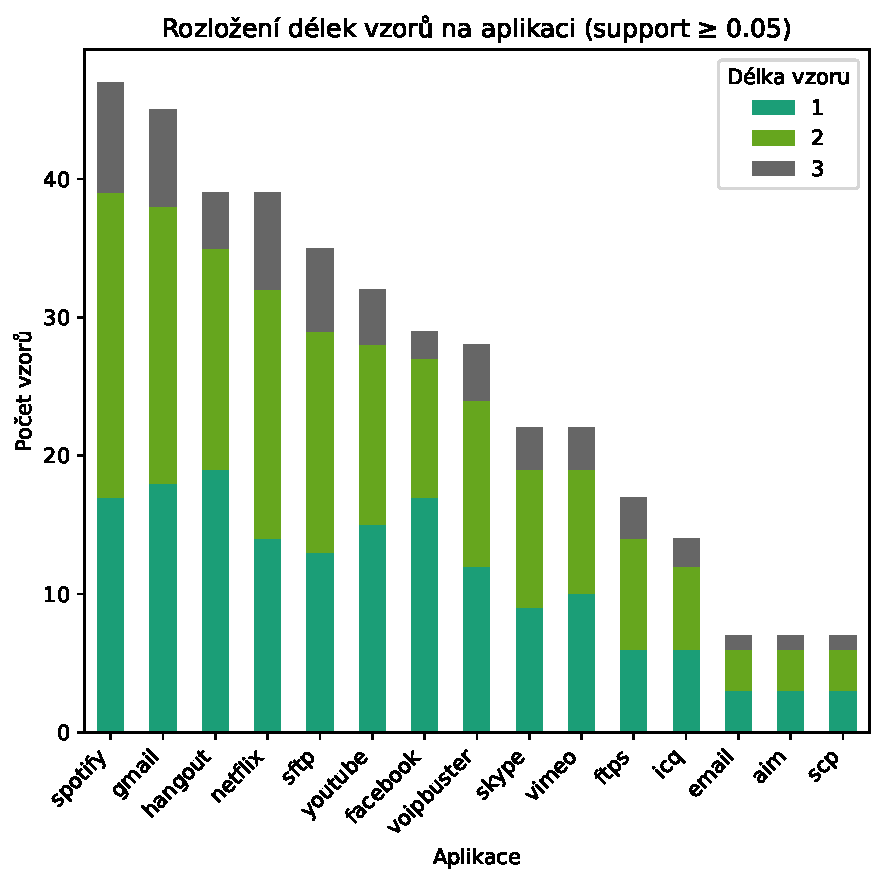
\includegraphics[width=\linewidth]{obrazky-figures/exps/pattern_lengths_0.05_iscx.pdf}

            \caption{Počet vzorů a~rozložení délek vzoru na~aplikaci pro~\texttt{iscx.csv} při~minimální podpoře 0.05.}
        \label{fig:appendix-}
    \end{minipage}
\end{figure}

\begin{figure}[H]
    \centering
    \begin{minipage}[t]{0.49\textwidth}
        \centering
    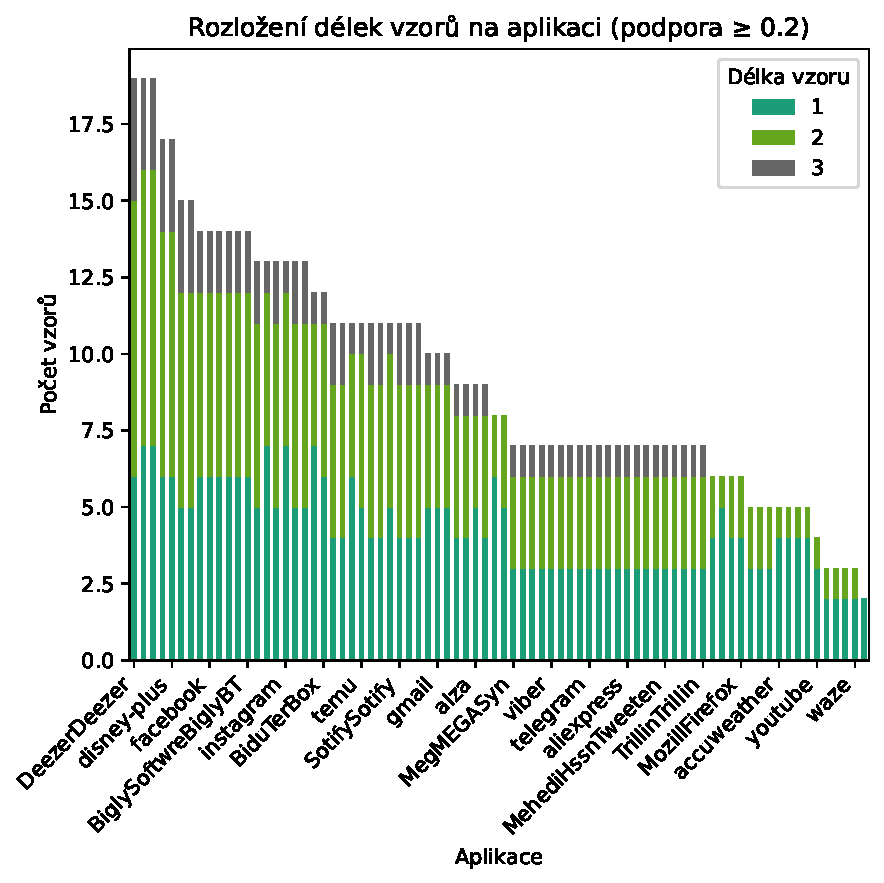
\includegraphics[width=\linewidth]{obrazky-figures/exps/pattern_lengths_0.2_mobile.pdf}
        \caption{Počet vzorů a~rozložení délek vzoru na~aplikaci pro~\texttt{mobile desktop apps raw.csv} při~minimální podpoře 0.2.}
    \label{fig:appendix-}
    \end{minipage}%
    \hfill
    \begin{minipage}[t]{0.49\textwidth}
       \centering
        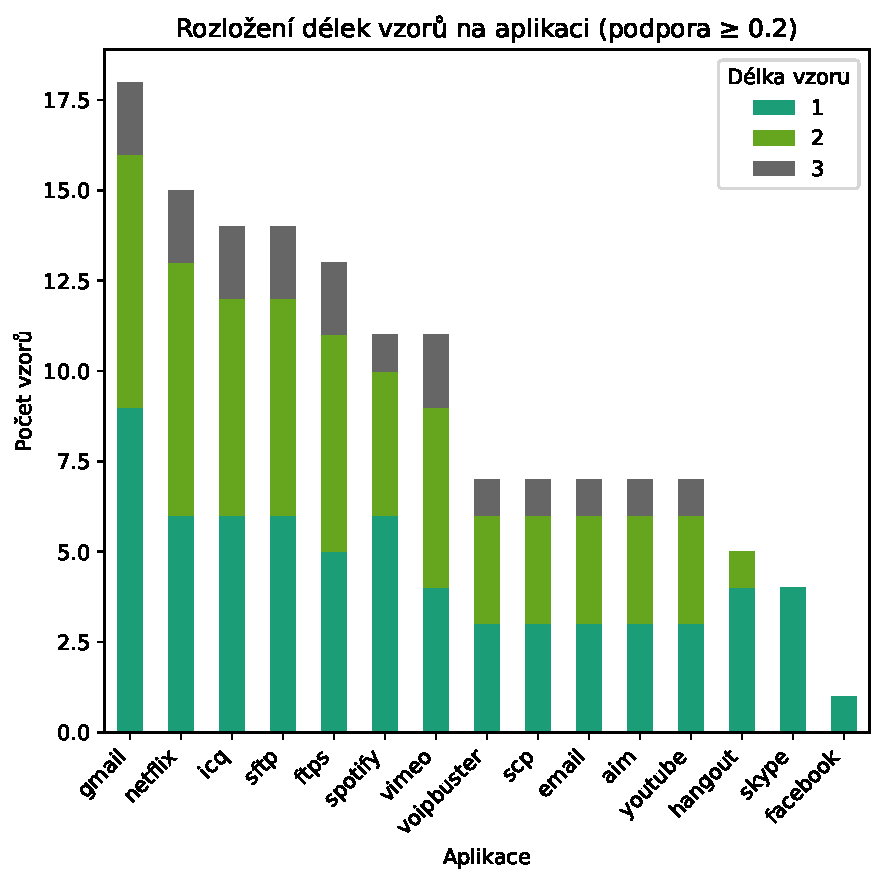
\includegraphics[width=\linewidth]{obrazky-figures/exps/pattern_lengths_0.2_iscx.pdf}

            \caption{Počet vzorů a~rozložení délek vzoru na~aplikaci pro~\texttt{iscx.csv} při~minimální podpoře 0.2.}
        \label{fig:appendix-}
    \end{minipage}
\end{figure}

\begin{figure}[H]
    \centering
     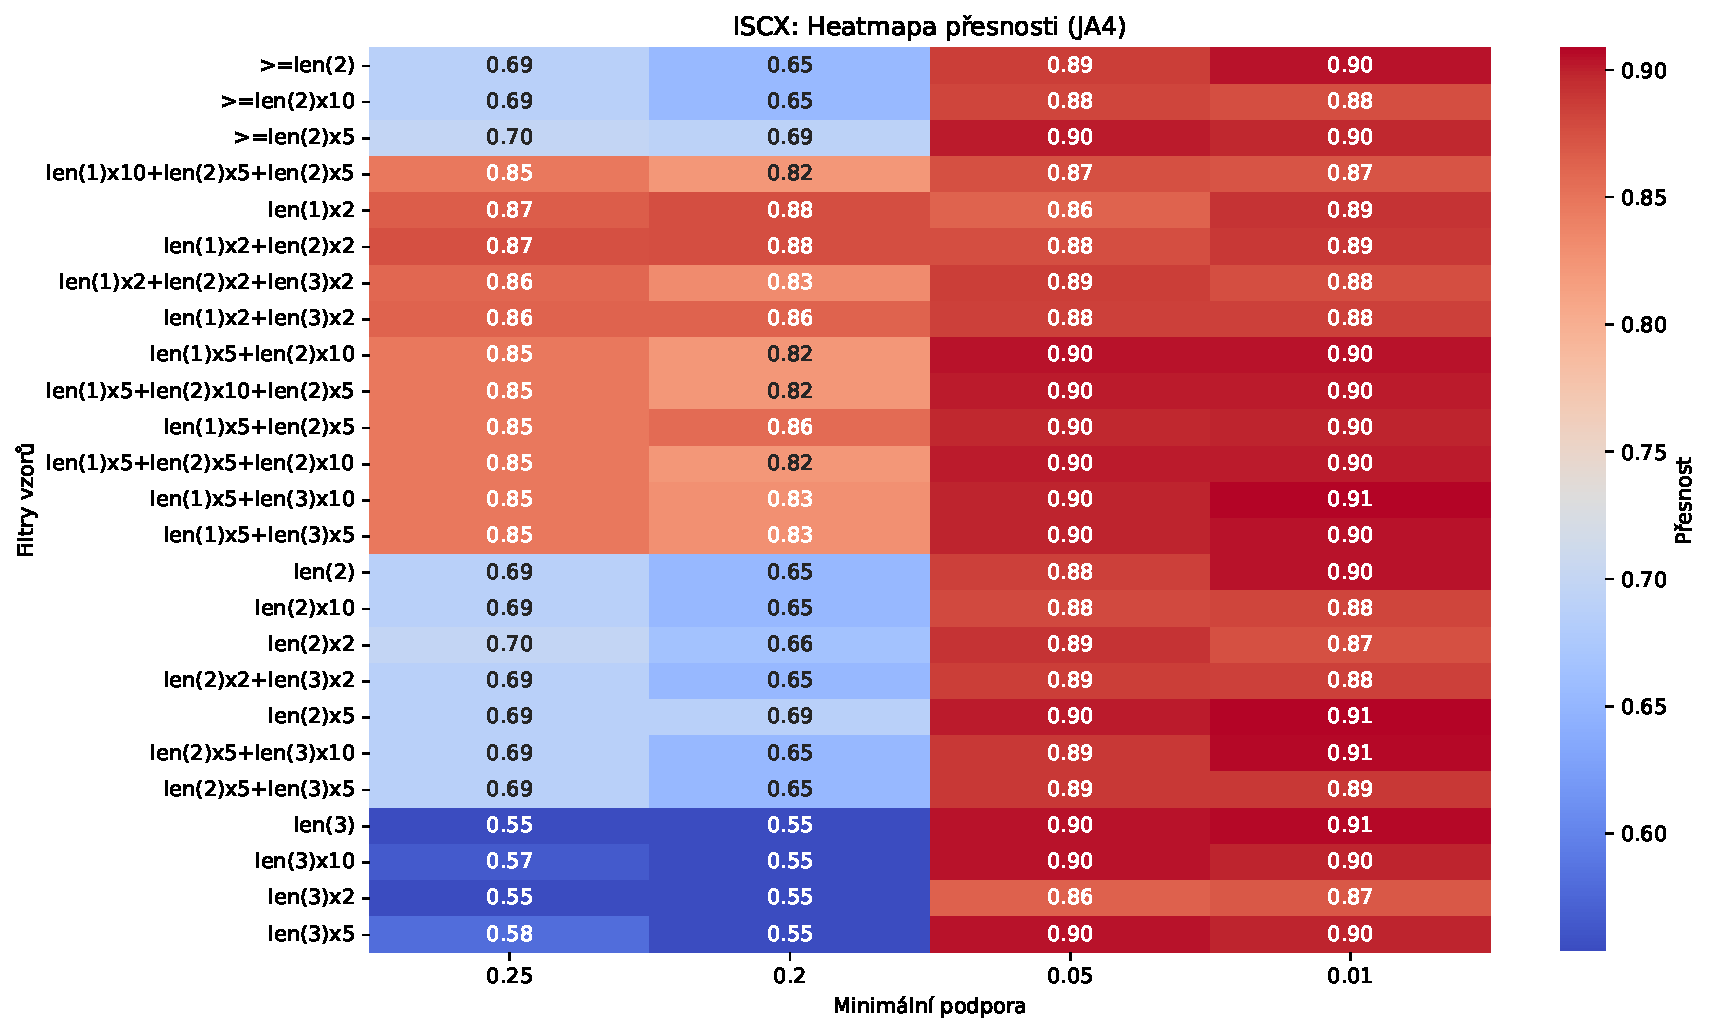
\includegraphics[angle=-90, width=0.8\textwidth]{obrazky-figures/exps/ex3-iscx-heatmap-JA4.pdf}
    \caption{Heatmapa zobrazuje testované kombinace otisků a~filtrů při~použití různých selekčních strategií nad~datovou sadou \texttt{iscx.csv}, konkrétně pro~kombinaci otisků \textit{JA4}. Barevné škálování reprezentuje dosaženou přesnost identifikace pro~každou konfiguraci.}
    \label{fig:appendix-heatmap-iscx-filter-ja4}
\end{figure}

\begin{figure}[H]
    \centering
    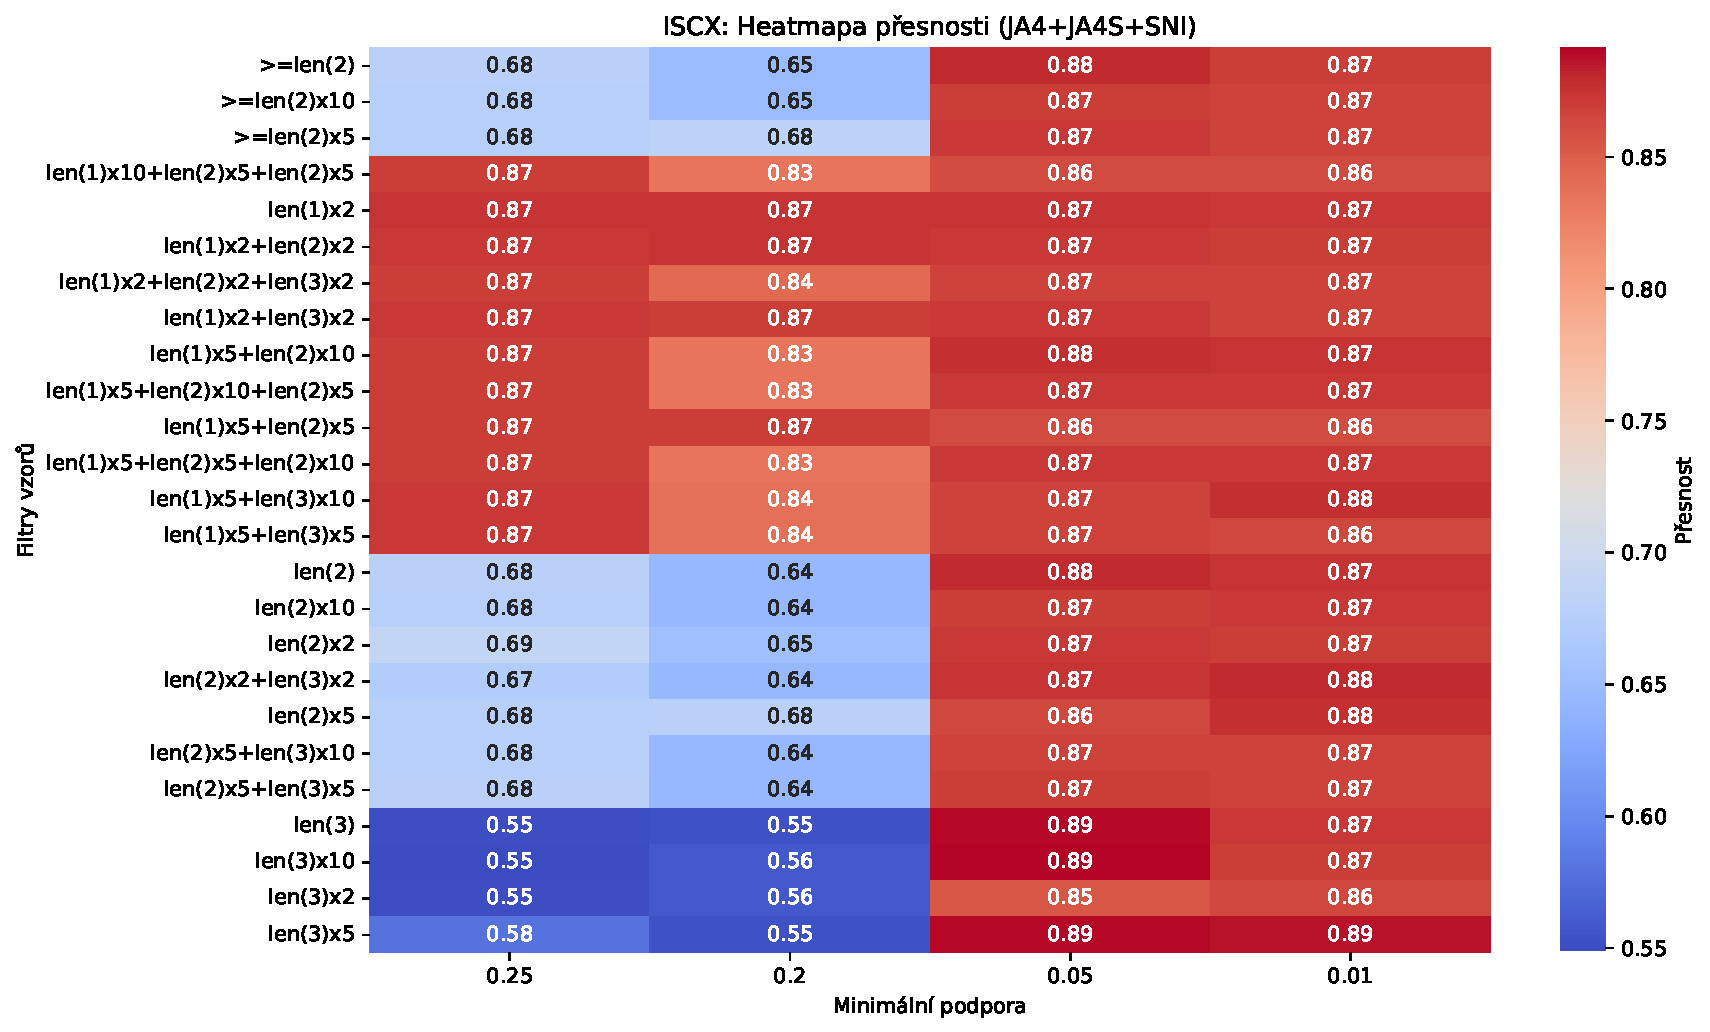
\includegraphics[angle=-90, width=0.8\textwidth]{obrazky-figures/exps/ex3-iscx-heatmap-JA4+JA4S+SNI.pdf}
    \caption{Heatmapa zobrazuje testované kombinace otisků a~filtrů při~použití různých selekčních strategií nad~datovou sadou \texttt{iscx.csv}, konkrétně pro~kombinaci otisků \textit{JA4+JA4S+SNI}. Barevné škálování reprezentuje dosaženou přesnost identifikace pro~každou konfiguraci.}
    \label{fig:appendix-heatmap-iscx-filter-ja4}
\end{figure}

\begin{figure}[H]
    \centering
    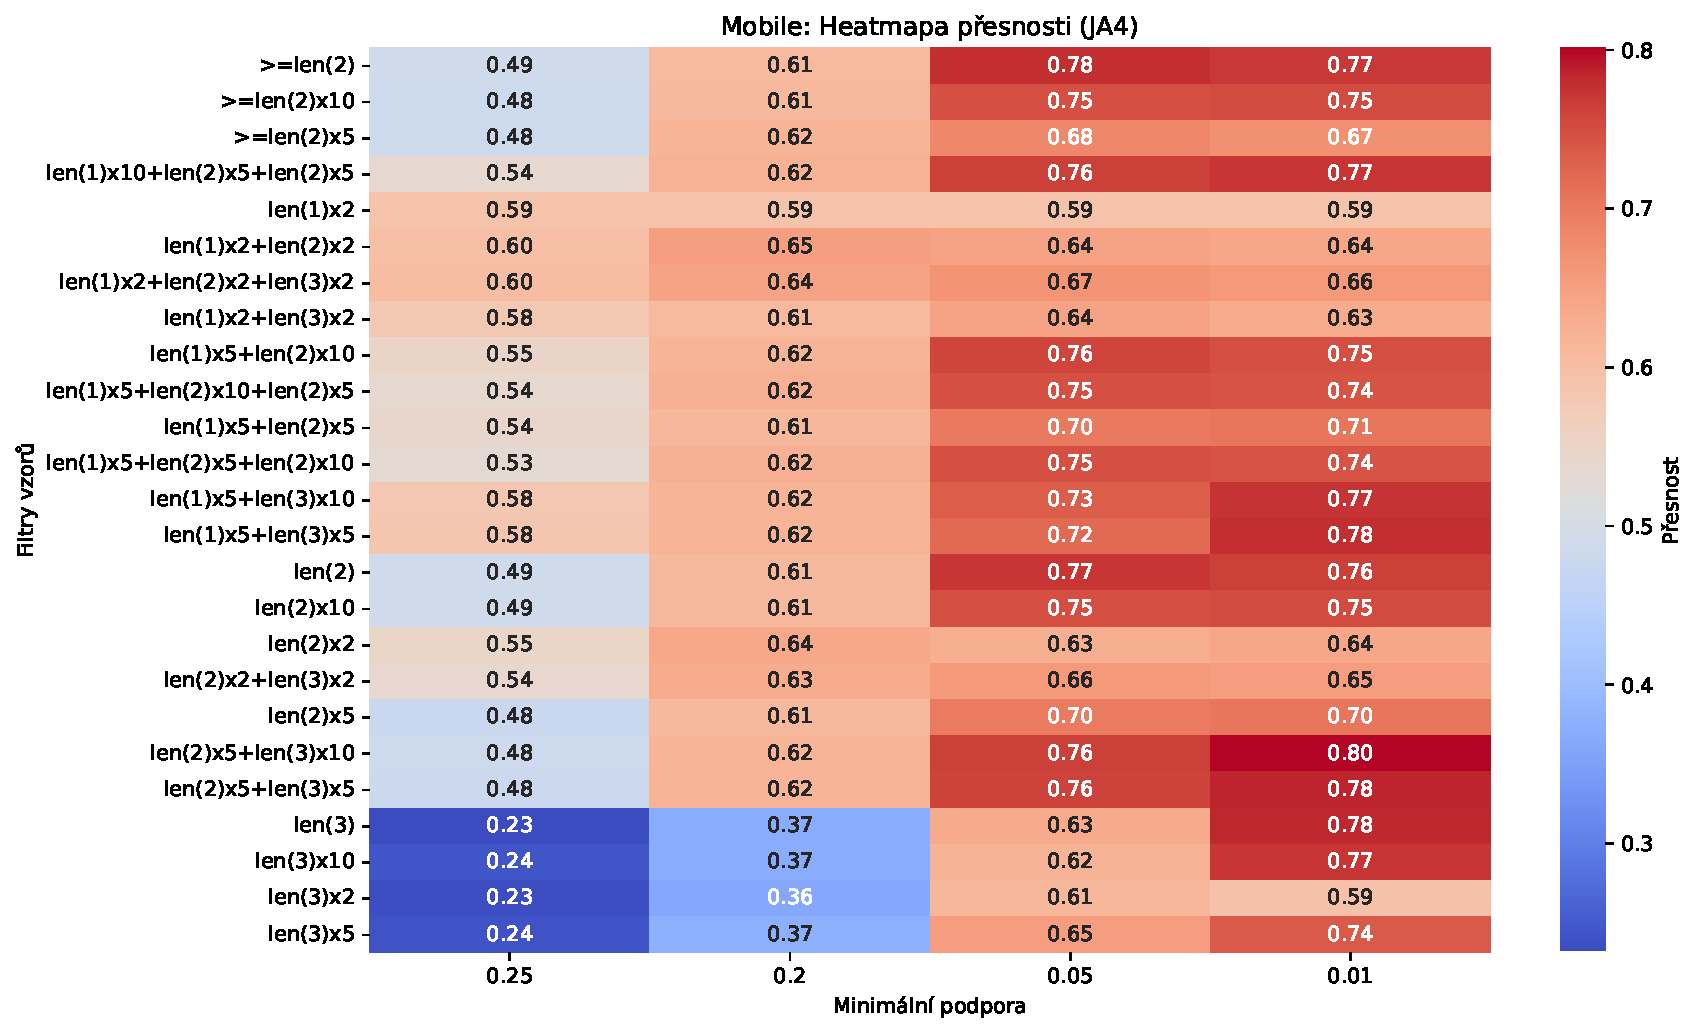
\includegraphics[angle=-90, width=0.8\textwidth]{obrazky-figures/exps/ex3-mobile-heatmap-JA4.pdf}
    \caption{Heatmapa zobrazuje testované kombinace otisků a~filtrů při~použití různých selekčních strategií nad~datovou sadou \texttt{mobile\_desktop\_apps\_raw.csv}, konkrétně pro~kombinaci otisků \textit{JA4}. Barevné škálování reprezentuje dosaženou přesnost identifikace pro~každou konfiguraci.}
    \label{fig:appendix-heatmap-iscx-filter-ja4}
\end{figure}

\begin{figure}[H]
    \centering
    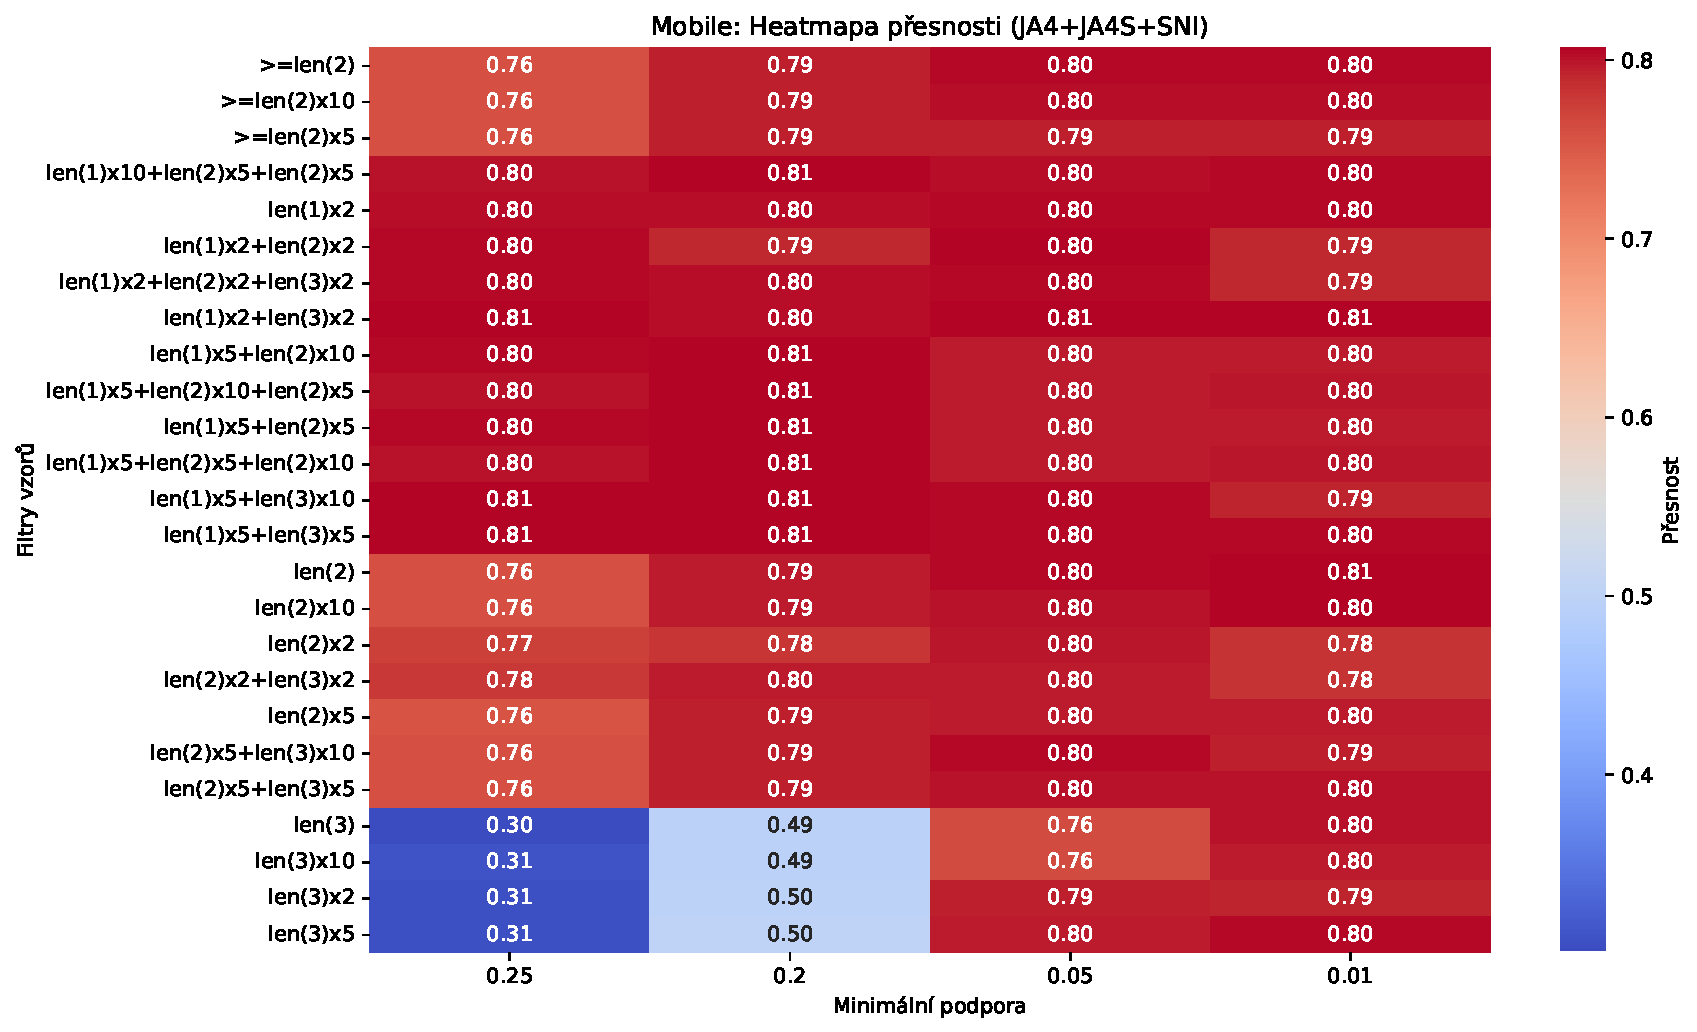
\includegraphics[angle=-90, width=0.8\textwidth]{obrazky-figures/exps/ex3-mobile-heatmap-JA4+JA4S+SNI.pdf}
    \caption{Heatmapa zobrazuje testované kombinace otisků a~filtrů při~použití různých selekčních strategií nad~datovou sadou \texttt{mobile\_desktop\_apps\_raw.csv}, konkrétně pro~kombinaci otisků \textit{JA4+JA4S+SNI}. Barevné škálování reprezentuje dosaženou přesnost identifikace pro~každou konfiguraci.}
    \label{fig:appendix-heatmap-iscx-filter-ja4}
\end{figure}
